\newpage
МРНТИ 31.23.01
\hfill {\bfseries \href{https://doi.org/10.58805/kazutb.v.3.24-449}{https://doi.org/10.58805/kazutb.v.3.24-449}}

\sectionwithauthors{Қ.А. Куртибай, Ә. Қаппасұлы, А.Ә. Үсенова, Е.Е. Жатканбаев, Ж.К. Жатканбаева, Н.Б. Молдагулова, Э.Б. Молдагулова}{ИЗУЧЕНИЕ СПОСОБОВ ЭФФЕКТИВНОГО ПОЛУЧЕНИЯ ЦЕЛЛЮЛОЗЫ ИЗ СТЕБЛЕЙ
ХЛОПЧАТНИКА ПРОИЗРОСТАЕМОЙ В ТУРКЕСТАНСКОЙ ОБЛАСТИ}

\begin{center}
{\bfseries \textsuperscript{1}Қ.А. Куртибай\envelope, \textsuperscript{1}Ә. Қаппасұлы, \textsuperscript{1}А.Ә. Үсенова, \textsuperscript{2}Е.Е. Жатканбаев, \textsuperscript{3}Ж.К. Жатканбаева, \textsuperscript{1}Н.Б. Молдагулова, \textsuperscript{1}Э.Б. Молдагулова}

\textsuperscript{1} ТОО «Научно-производственный центр экологической и
промышленной биотехнологии», Астана, Казахстан,

\textsuperscript{2} Казахский университет технологии и бизнеса имени К.
Кулажанова, Астана, Казахстан,

\textsuperscript{3} Евразийский Национальный Университет имени Л.Н.
Гумилёва, Астана, Казахстан
\end{center}
\envelope Корреспондент-автор: kurtibayqb@gmail.com


В Казахстане тема переработки хлопковых отходов очень актуальна в
современных условиях. Учитывая, что Казахстан является одним из
крупнейших производителей хлопка в мире, на повестке дня стоит вопрос
утилизации большого количества стеблей хлопчатника и других отходов,
образующихся после сбора хлопка. Неэффективная утилизация этих отходов
приводит к серьезным экологическим проблемам, таким как загрязнение
почвы и воды, а также выбросы парниковых газов при их сжигании. Кроме
того, отсутствие эффективных методов переработки лишает страну
возможности использовать хлопковые отходы для производства ценной
продукции, такой как целлюлоза, ограничивая экономический потенциал
региона. Таким образом, разработка и внедрение новых эффективных
технологий переработки хлопковых отходов в Казахстане имеет не только
экологически и экономически актуальное, но и стратегическое значение для
устойчивого развития страны. Переработка стеблей хлопчатника и других
отходов в лигноцеллюлозу и целлюлозу может стать источником новых
экономических возможностей как для мира, так и для Казахстана, где
интенсивно выращивается хлопок. Переработка стеблей хлопка и других
хлопковых остатков помогает сократить количество отходов, которые обычно
выбрасываются в мусор или массово сжигаются после сбора хлопка. Решением
этих проблем может стать переработка этих отходов и получение из них
ценной продукции во избежание глобального потепления и других негативных
последствий, угрожающих окружающей среде.

{\bfseries Ключевые слова:} стебель хлопчатника, целлюлоза, лигноцеллюлоза,
щелочная варка, делигнификация, число Каппа.

\sectionheading{ТҮРКІСТАН ОБЛЫСЫНДА ӨСІРІЛЕТІН МАҚТА САБАҒЫНАН ЦЕЛЛЮЛОЗАНЫ
ТИІМДІ АЛУ ЖОЛДАРЫН ЗЕРТТЕУ}

\begin{center}
{\bfseries \textsuperscript{1}Қ.А. Куртибай\envelope, \textsuperscript{1}Ә.
Қаппасұлы, \textsuperscript{1}А.Ә. Үсенова, \textsuperscript{2}Е.Е.
Жатканбаев, \textsuperscript{3}Ж.К. Жатканбаева, \textsuperscript{1}Н.Б.
Молдагулова, \textsuperscript{1}Э.Б. Молдагулова}

«Экологиялық және өнеркәсіптік биотехнологияның ғылыми-өндірістік
орталығы» ЖШС, Астана, Қазақстан,

\textsuperscript{2} Қ. Құлажанов атындағы Қазақ технология және бизнес
университеті, Астана, Қазақстан,

\textsuperscript{3} Л.Н. Гумилев атындағы Еуразия Ұлттық Университеті,
Астана, Қазақстан,

e-mail: kurtibayqb@gmail.com
\end{center}

Қазақстанда мақта қалдықтарын қайта өңдеу тақырыбы қазіргі контексте өте
өзекті. Қазақстан әлемдегі ең ірі мақта өндірушілердің бірі болып
табылатындығын ескере отырып, мақта жинағаннан кейін пайда болатын мақта
сабақтарының және басқа да қалдықтардың үлкен көлемін утилизациялау
мәселесі күн тәртібінде тұр. Бұл қалдықтарды тиімсіз утилизациялау
топырақ пен судың ластануы, сондай-ақ оларды жағу кезінде парниктік
газдар шығарындылары сияқты маңызды экологиялық мәселелерге әкеледі.
Сонымен қатар, өңдеудің тиімді әдістерінің болмауы елді мақта
қалдықтарын целлюлоза сияқты құнды өнімдерді өндіру үшін пайдалану
мүмкіндігінен айырады, бұл аймақтың экономикалық әлеуетін шектейді.
Осылайша, Қазақстанда мақта қалдықтарын қайта өңдеудің жаңа
технологияларын әзірлеу және енгізу экологиялық және экономикалық
тұрғыдан өзекті болып қана қоймай, елдің тұрақты дамуы үшін стратегиялық
маңызы бар. Мақта сабақтарын және басқа да қалдықтарды лигноцеллюлоза
мен целлюлозаға өңдеу ғалам үшін де, мақта қарқынды өсірілетін аймақ
үшін де жаңа экономикалық мүмкіндіктердің көзі болуы мүмкін. Мақта
сабақтарын және оның басқа да қалдықтарын қайта өңдеу әдетте мақта
жиналғаннан кейін қоқыс ретінде тасталатын немесе жаппай өртелетін
қалдықтарды азайтуға көмектеседі. Бұл проблемалардың шешімі жаһандық
жылынуды және қоршаған ортаға қауіп төндіретін басқа да жағымсыз
әсерлерді болдырмау үшін осы қалдықтарды қайта өңдеу және олардан құнды
өнімдер алу болуы мүмкін.

{\bfseries Түйін сөздер:} мақта сабағы, целлюлоза, лигноцеллюлоза, сілтілік
қайнату, делигнификация, Каппа саны.

\sectionheading{STUDY OF METHODS FOR EFFICIENT PRODUCTION OF CELLULOSE FROM
COTTON STALKS GROWN IN TURKESTAN REGION}

\begin{center}
{\bfseries \textsuperscript{1}K.A. Kurtibay\envelope, \textsuperscript{1}A.
Kappassuly, \textsuperscript{1}A.A. Ussenova, \textsuperscript{2}Ye.Ye.
Zhatkanbayev,}

{\bfseries \textsuperscript{3}Zh.K. Zhatkanbayeva, \textsuperscript{1}N.B.
Moldagulova, \textsuperscript{1}E.B. Moldagulova}

\textsuperscript{1} «Scientific and Production Center of Ecological and
Industrial Biotechnology» LLP, Astana, Kazakhstan,

\textsuperscript{2} Kazakh University of Technology and Business named
after K. Kulazhanov, Astana, Kazakhstan,

\textsuperscript{3} L.N. Gumilyev Eurasian National University, Astana,
Kazakhstan,

e-mail: kurtibayqb@gmail.com
\end{center}

In Kazakhstan, the topic of cotton waste recycling is very relevant in
modern conditions. Given that Kazakhstan is one of the largest cotton
producers in the world, the issue of utilization of a large amount of
cotton stalks and other waste generated after cotton harvesting is on
the agenda. Inefficient utilization of these wastes leads to serious
environmental problems, such as soil and water pollution, as well as
greenhouse gas emissions from their incineration. In addition, the lack
of efficient processing methods deprives the country of the opportunity
to utilize cotton waste to produce valuable products such as pulp,
limiting the economic potential of the region. Thus, the development and
implementation of new efficient technologies for processing cotton waste
in Kazakhstan is not only environmentally and economically relevant, but
also of strategic importance for the sustainable development of the
country. Processing of cotton stalks and other wastes into
lignocellulose and cellulose can become a source of new economic
opportunities both for the world and for Kazakhstan, where cotton is
intensively grown. Recycling cotton stalks and other cotton residues
helps to reduce the amount of waste that is usually disposed of in
garbage or mass burned after cotton harvesting. The solution to these
problems could be to recycle these wastes and get valuable products out
of them to avoid global warming and other negative effects that threaten
the environment.

{\bfseries Key words:} cotton stalk, cellulose, lignocellulose, alkaline
pulping, delignification, Kappa number.

\begin{multicols}{2}
{\bfseries Введение.} Растущая проблема нехватки энергии в мире и быстрое
истощение запасов ископаемого топлива, а также такие экологические
проблемы, как глобальное потепление, кислотные дожди и городской смог,
послужили толчком к активным исследованиям в области альтернативных и
возобновляемых источников энергии {[}1{]}. Все большее внимание
уделяется сохранению экологических систем. Большинство синтетических
полимеров сегодня производятся из нефтехимических продуктов и редко
подвергаются биологическому разложению. Постоянное использование этих
полимеров значительно загрязняет окружающую среду и наносит вред дикой
природе, когда они выбрасываются в природу {[}2{]}. Например,
неразлагающиеся пластиковые пакеты негативно влияют на морских
обитателей. Широко признано, что использование долговечных полимеров в
изделиях с коротким сроком службы, например, в машиностроении, упаковке,
общественном питании, хирургии и гигиене, нецелесообразно. Кроме того,
сжигание пластиковых отходов создает экологические проблемы из-за
выделения токсичных веществ, таких как диоксин. Биоразлагаемые полимеры
уже давно рассматриваются как потенциальное решение, поскольку они могут
помочь преодолеть ограниченность нефтехимических ресурсов. Использование
экологически чистых сельскохозяйственных ресурсов вместо ископаемого
топлива и газа также поможет сократить выбросы CO\textsubscript{2}
{[}3{]}.

При выращивании хлопчатника образуются значительные растительные
остатки, вес которых зачастую в три-пять раз превышает вес производимого
хлопчатника {[}4{]}. Эти остатки, состоящие в основном из стеблей, дают
примерно 2,5-3,5 тонны на акр возделываемого хлопчатника, что зависит от
используемой уборочной техники {[}5{]}. В настоящее время распространена
практика сжигания стеблей хлопчатника на поле из-за опасений передачи
болезней будущим посевам хлопчатника. Однако в стеблях содержится
большое количество целлюлозы, что побуждает исследовать возможность их
использования в различных областях, таких как производство бумаги,
промышленного топлива, композитных материалов и регенерации целлюлозы
для производства вискозы {[}4,6{]}.

Стебель хлопчатника является остаточным продуктом хлопководства и
классифицируется как возобновляемая лигноцеллюлозная биомасса. Благодаря
содержанию целлюлозы от 32 до 46 \% и гемицеллюлозы от 20 до 28 \%,
стебель хлопчатника является перспективным сырьем для переработки
целлюлозы {[}7{]}.

В последнее время для переработки лигноцеллюлозной биомассы все большую
популярность приобретают методы предварительной обработки на основе
кислот и щелочей, каждый из которых использует различные механизмы
разрушения клеточных стенок. Кислотная предварительная обработка обычно
разрушает компоненты гемицеллюлозы и делает целлюлозу более податливой
для ферментативного расщепления {[}8{]}. Обычно для этого процесса
используются разбавленные кислоты, такие как серная, азотная и соляная,
что объясняется их экономичностью и экологическими преимуществами
{[}8,9{]}. Предварительная обработка щелочью разрушает эфирные связи,
соединяющие лигнин и ксилан, удаляет лигнин, вызывает набухание
целлюлозы и частично декристаллизует целлюлозу {[}10{]}. Лигноцеллюлоза,
как самый распространенный и воспроизводимый ресурс, обнаружила
потенциал как сырье для производства топлива и химических веществ с
добавленной стоимостью {[}11{]}, {[}12{]}. Ее состав в основном включает
три основных структурных компонента: целлюлозу, гемицеллюлозу и лигнин.
Обычно сухая лигноцеллюлоза содержит примерно 40-50\% целлюлозы,
20-30\% гемицеллюлозы и 20-35\% лигнина {[}13{]}. Очевидно, что
целлюлоза является наиболее распространенным компонентом лигноцеллюлозы
и состоит из молекул D-глюкозы, соединенных между собой
1,4-β-гликозидными связями {[}13{]}. Все эти усилия по повышению
ценности стеблей хлопчатника становятся все более необходимыми в борьбе
с загрязнением окружающей среды и глобальным дефицитом энергии.

В Казахстане большое значение имеют исследования по переработке отходов,
такие как стебли хлопчатника. Разработка эффективных методов утилизации
этих отходов не только способствует снижению негативного воздействия на
окружающую среду и повышению экологической устойчивости региона, но и
открывает новые возможности для экономического развития.

{\bfseries Методы и материалы.} В качестве объекта исследования в данной
работе были выбраны отходы хлопчатника, выращиваемого в Туркестанском
регионе Республики Казахстан, а именно стебли хлопчатника. Объект
исследования был собран с поля, где выращивался хлопчатник, очищен от
листьев, хлопчатника, шелухи и корней стеблей хлопчатника, и
первоначальный процесс сушки проводился в тени при атмосферной
температуре в течение 7-10 дней. Сухие стебли общим весом 10 кг были
собраны для переработки стеблей хлопчатника для исследовательской
работы. Каждый стебель хлопчатника был обрезан так, чтобы его длина
составляла 7-10 см (Рисунок 1 а). Стебли хлопчатника, предварительно
собранные и высушенные в тени в течение недели, измельчаются до мелких
частиц. Измельченную пробу сушат до постоянной массы в конвекционной
печи при температуре 105°С (Рисунок 1 б).
\end{multicols}

\begin{figure}[H]
    \centering
    \begin{subfigure}[b]{0.32\textwidth}
        \centering
        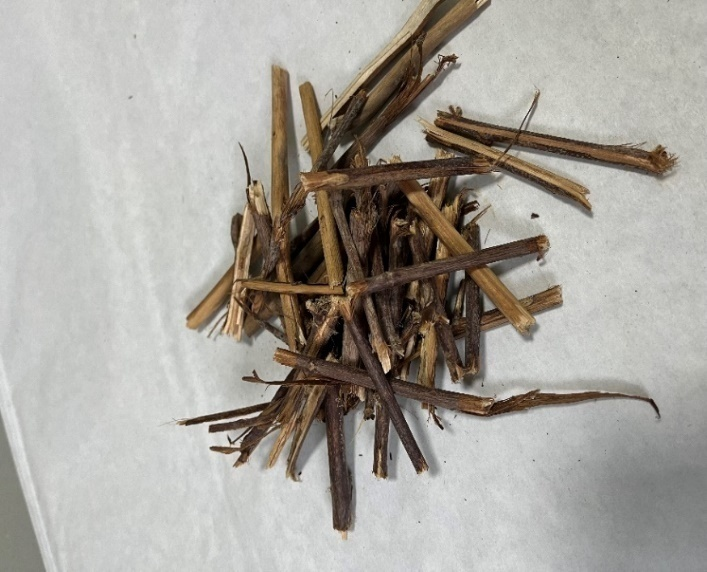
\includegraphics[height=0.9\textwidth]{assets/75}
        \caption*{а}
    \end{subfigure}
    \hspace{2em}
    \begin{subfigure}[b]{0.32\textwidth}
        \centering
        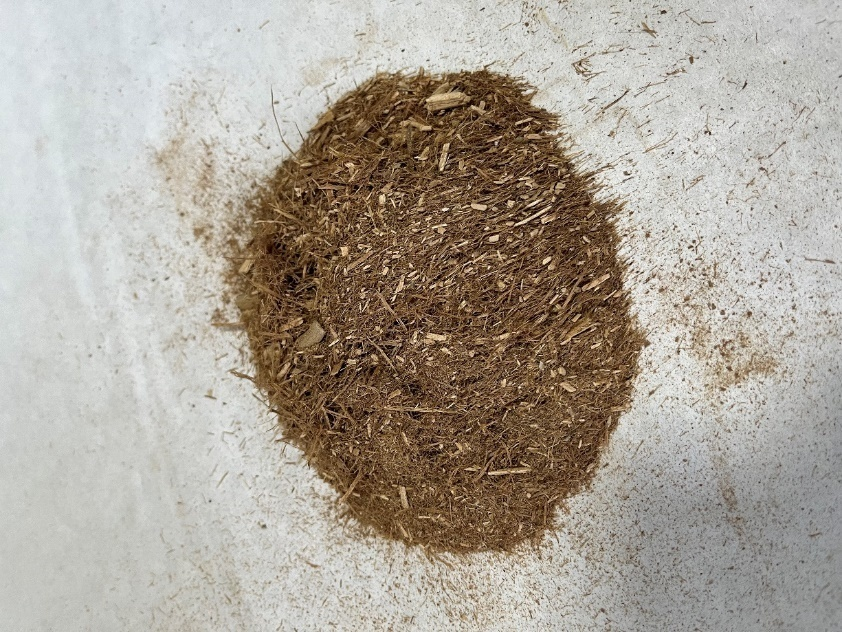
\includegraphics[height=0.9\textwidth]{assets/76}
        \caption*{б}
    \end{subfigure}
    \caption*{Рис. 1 - а- стебли хлопчатника, б-измельченный образец из стеблей хлопчатника}
\end{figure}

\begin{multicols}{2}
1. \emph{Получение целлюлозы интегрированным методом экстракции и делигнификации}

Порошок стеблей хлопчатника обрабатывали хлороформом (2:1 по объему) для
удаления масел и восков путем экстракции в аппарате Сокслета в течение 6
часов, а затем сушили в конвекционной печи при температуре 110°C в
течение 8 часов до постоянной массы. Высушенный порошок стеблей
хлопчатника обрабатывают 2 н HCl при температуре 40-60°C в течение 3-4
часов. Затем реакционную смесь фильтруют и несколько раз промывают
дистиллированной водой до нейтральной среды. Наконец, промытый остаток в
фильтре делигнифицируют 20\% водным раствором гидроксида натрия при
температуре 120°C (1,5 бар) в автоклаве в течение 2 часов {[}14{]}.

2. \emph{Получение целлюлозы путем щелочной варки}

Для определения влияния концентрации щелочи на выход целлюлозы
использовались 10\%, 15\% и 20\% растворы гидроксида натрия. Кроме того,
в целях достижения высокой степени делингинификации и обеспечения
высокого выхода целлюлозы процесс проводился с помощью
автоклав-стерилизатора (Казахстан) при температуре 120°C и при давлении
1,5 бар. Для определения зависимости выхода целлюлозы от времени
проводили процесс щелочной варки стеблей хлопчатника (5:1) в течение 2-4
часов. После завершения процесса раствор фильтровали и промывали
дистиллированной водой до тех пор, пока значение pH остатка не показало
нейтральную среду. Позже целлюлозу, полученную путем щелочной варки из
стебля хлопчатника, сушили в конвекционной печи при температуре 105°C до
постоянной массы, высушенный образец хранили в эксикаторе с прокаленным
хлоридом кальция для последующих экспериментов.

3. \emph{Процесс обесцвечивания}

Процесс обесцвечивания полученной сырой целлюлозы проводился путем
смешивания с 3\% раствором H\textsubscript{2}O\textsubscript{2} в
соотношении 2:1 в течение 3 часов на водяной бане при температуре 80°C.

4. \emph{Определение выхода целлюлозы}

Выход целлюлозы, полученной из стеблей хлопчатника двумя методами,
определяли по следующему уравнению:

\begin{equation}
\omega,\ \% = \ \frac{m_{2}}{m_{1}}*100
\end{equation}

где,

\emph{ω, \%} - выход целлюлозы;

\emph{m\textsubscript{1}} - исходная масса образца;

\emph{m\textsubscript{2}} - масса полученной целлюлозы.

4. \emph{Определение числа Каппа}

Число Каппа является показателем степени делигнификации целлюлозы или ее
обесцвечивания. Определение числа Каппа целлюлозы проводили методом
титрования по международному стандарту ISO 302:2015 «Целлюлоза.
Определение числа Каппа». Настоящий международный стандарт
распространяется на все виды химической и полухимической целлюлозы с
числом Каппа в диапазоне от 1 до 100.

5. \emph{Исследование методом ИК-Фурье спектроскопии}

Изоляты целлюлозы, полученные в ходе исследования, были проанализированы
с использованием метода ослабленного полного отражения (ATR) для
определения химического состава с помощью ИК-Фурье-спектрометра IRSpirit
(Shimadzu, Япония). Спектры ИК-Фурье регистрировались в диапазоне длин
волн 400-4000 см\textsuperscript{-1} со спектральным разрешением 4
см\textsuperscript{-1}. Образцы были проанализированы на
ИК-Фурье-спектрометре по таблетированному методу с бромидом калия.
Соотношение образца к KBr составляет 1:10.

{\bfseries Результаты и обсуждения.}

6. \emph{Получение целлюлозы интегрированным методом экстракции и делигнификации}

Являясь наиболее распространенным и возобновляемым источником,
лигноцеллюлоза является потенциальным сырьем для производства
дорогостоящего топлива и химикатов. В основном он состоит из трех
основных структурных компонентов: целлюлозы, гемицеллюлозы и лигнина.
Обычно сухая лигноцеллюлоза состоит примерно из 40-50\% целлюлозы,
20-30\% гемицеллюлозы и 20-35\% лигнина. Целлюлоза, очевидно, является
наиболее распространенным компонентом лигноцеллюлозы, которая состоит из
единиц D-глюкозы, связанных 1,4-β-гликозидными связями. На практике
целлюлозу можно превратить путем пиролиза в полезные химические
вещества, такие как маннит, фурфурол и левоглюкозенон, или топливо,
включая целлюлозный этанол и биотопливо.

В процессе переработки биомассы деградация целлюлозы сопровождается
деградацией гемицеллюлозы, лигнина, масел и восков, что усложняет
процесс. Поэтому необходимо выделить из лигноцеллюлозной биомассы
основной компонент - целлюлозу и изучить продукты ее разложения. На
сегодняшний день сообщалось о различных методах разделения, таких как
паровой взрыв, микроволновая экстракция, обработка неорганическими
кислотами, обработка щелочью и методы ионной жидкости. Удаление масел и
восков осуществляется с помощью органических растворителей.

В этом исследовании целлюлозу экстрагировали из стеблей хлопчатника с
использованием соляной кислоты и гидроксида натрия для удаления
гемицеллюлозы и лигнина, что является самым простым и экономичным
методом {[}14{]}.

Образец порошка стеблей хлопчатника массой 100 г экстрагировали
хлороформом (2:1 по объему) в течение 6 часов в аппарате Сокслета для
удаления масел и воска (рис. 9), а затем сушили в конвекционной печи при
110°C в течение 8 часов. до постоянной массы. Масса высушенного образца
после экстракции составила 96,4 г.

Для удаления гемицеллюлозы и лигнина обезжиренный порошок высушенных
стеблей хлопчатника обрабатывают 2 M HCl при температуре 40-60°С в
течение 3-4 часов. Реакционную смесь затем фильтруют и остаток на
фильтре несколько раз промывают дистиллированной водой до нейтральной
реакции. Наконец, промытый выше остаток делигнифицируют 20\% водным
раствором гидроксида натрия в автоклаве при 120°C (1,5 бар) в течение 2
часов. На рисунке 2 показана сырая целлюлоза из обесцвеченных стеблей
хлопчатника после обработки кислотой и щелочью.

Выход целлюлозы из делигнифицированных стеблей хлопчатника после
кислотно-щелочной обработки составил 46,8\%. Выход продукта рассчитывали
по уравнению (1).

Полученную целлюлозу охарактеризовали методом ИК-Фурье-спектроскопии. С
целью изучения чистоты полученной целлюлозы исследовали так же ИК
спектры исходного образца (Рисунок 3-4).
\end{multicols}

\begin{figure}[H]
	\centering
	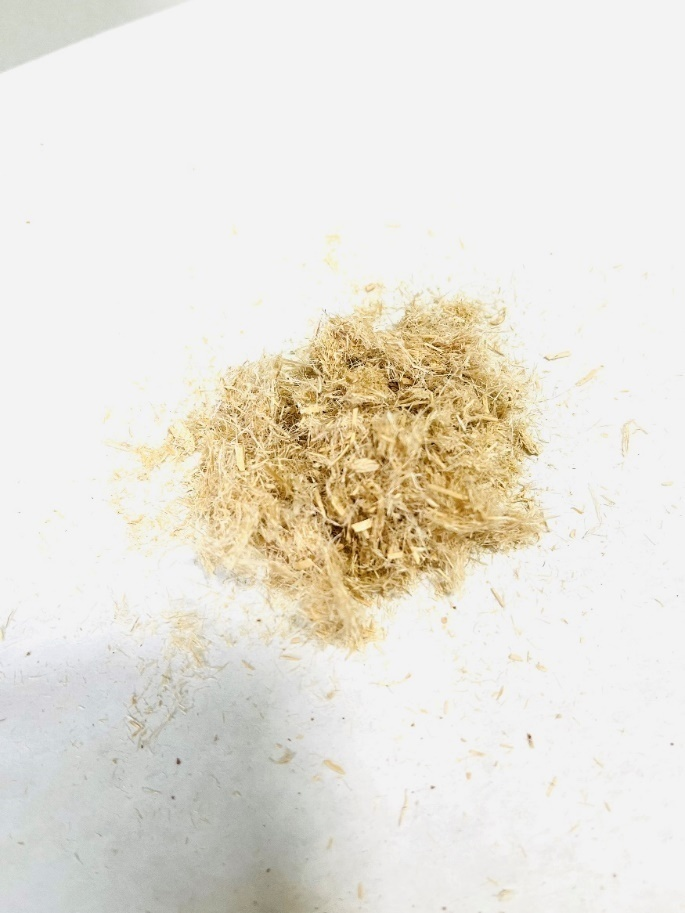
\includegraphics[width=0.3\textwidth]{assets/77}
	\caption*{Рис. 2 - Обесцвеченная целлюлоза из стеблей хлопчатника}
\end{figure}

\begin{multicols}{2}
Как видно из ИК-спектров на спектрограммах, полученные спектры целлюлозы
были аналогичны спектрам стеблей хлопчатника, за исключением полос при
1691 см\textsuperscript{-1} и 1550 см\textsuperscript{-1}, которые были
отнесены к поглощению карбонильных растяжении эфиров или карбоксильных
групп в гемицеллюлозе и колебания ароматического скелета в лигнине.
Сильное поглощение при 3392 см\textsuperscript{-1} и 2905
см\textsuperscript{-1} было приписано длинным колебаниям O-H и C-H в
целлюлозе соответственно. Поглощение около полоса 1635
см\textsuperscript{-1} указывает на изгибный режим поглощенной воды,
поскольку чистая целлюлоза обладает малыми гигроскопическими свойствами.
Поглощение при 1040 см\textsuperscript{-1} отнесено к валентным
колебаниям эфирных связей С-О-С. Небольшая резкая полоса при 898
см\textsuperscript{-1} характерна для поглощения β-гликозидных связей
между моносахаридами целлюлозы, указывая на то, что глюкоза, основная
цепь целлюлозы, связана с β-гликозидной связью.
\end{multicols}

\begin{figure}[H]
	\centering
	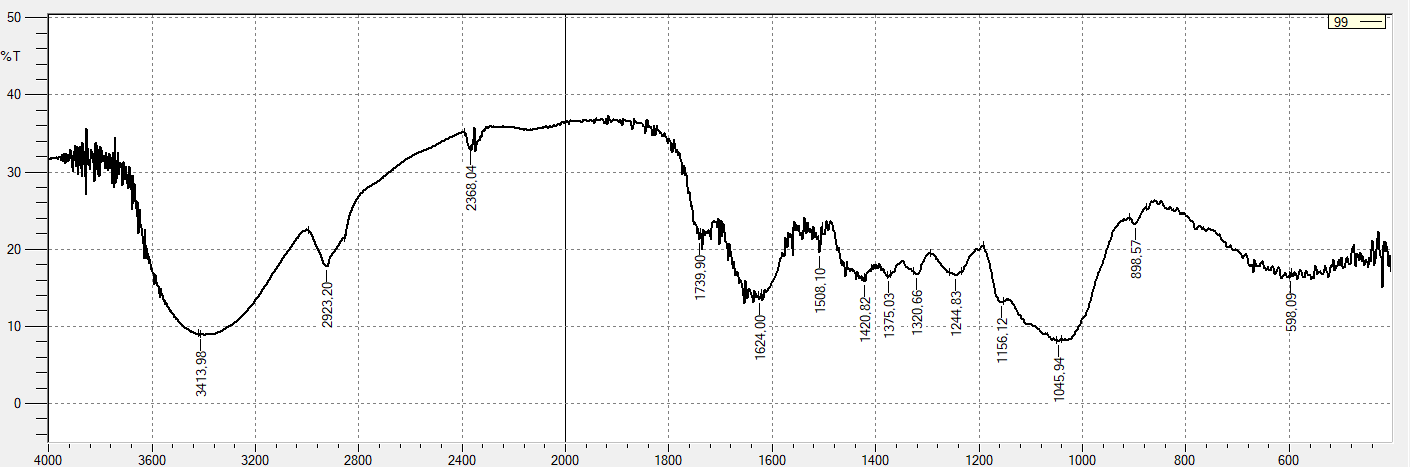
\includegraphics[width=0.8\textwidth]{assets/78}
	\caption*{Рис. 3 - ИК спектрограмма исходного образца}
\end{figure}

\begin{figure}[H]
	\centering
	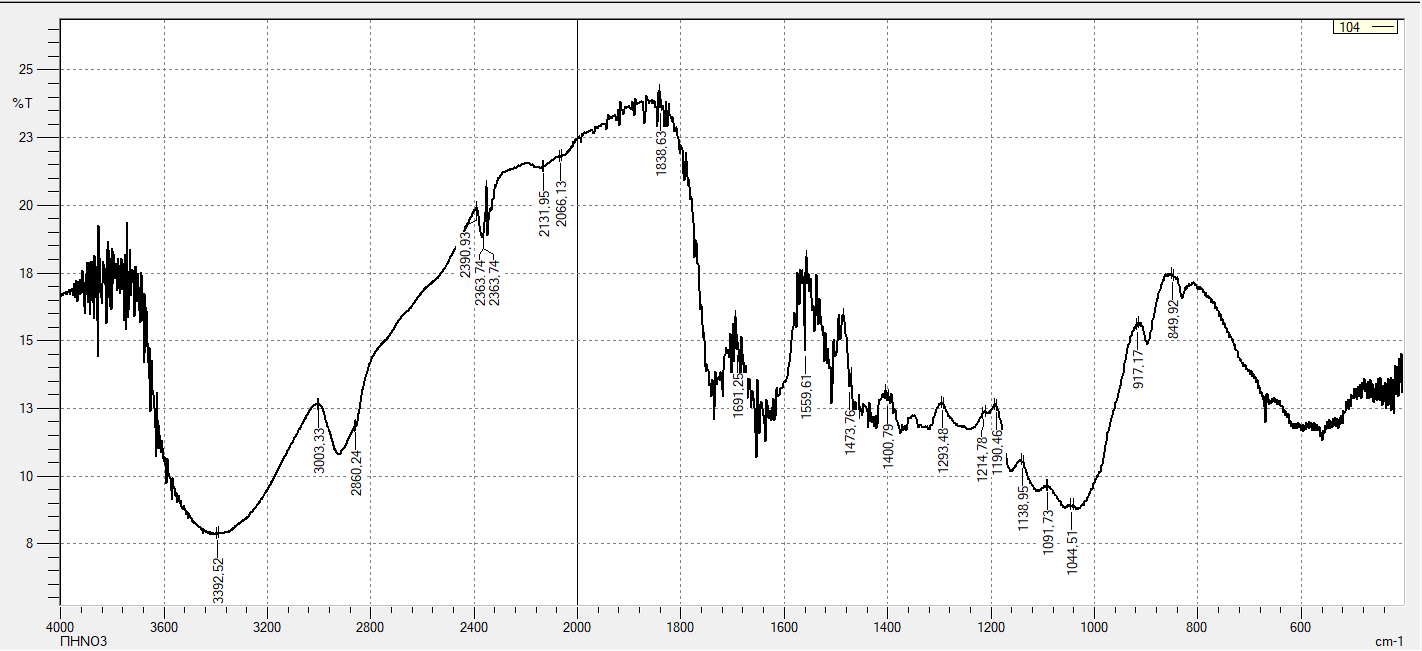
\includegraphics[width=0.8\textwidth]{assets/79}
	\caption*{Рис. 4 - ИК спектрограмма целлюлозы полученной по интегрированному методу экстракции и делигнификации}
\end{figure}

\begin{multicols}{2}
Таким образом, предварительная экстракция органическим растворителем
предотвратила удаление масел и восков, которые могут помешать дальнейшей
работе в нашем исследовании. А обработка кислотными и щелочными
растворами позволила избавиться от лигнина и гемицеллюлозы из стеблей
хлопчатника, которые в основном лигноцеллюлозные. Стоит отметить, что
щелочная вырка по нашему методу осуществляется в автоклаве при давлении
1,5 бар. Это, наряду с постепенным удалением других мешающих веществ,
способствовало увеличению выхода целлюлозы. В ходе
ИК-Фурье-спектроскопического анализа было установлено, что полученная
целлюлоза связана β-гликозидными связями, а наличие полос, характерных
для гидроксильных групп, также характеризовало наличие гигроскопических
свойств чистой целлюлозы.

\emph{2. Получение целлюлозы путем щелочной варки}

Щелочная варка, используемое в качестве предварительной обработки,
представляет собой процесс, при котором волокна подвергаются воздействию
гидроксида натрия или других щелочных реагентов при высоких
температурах. Этот процесс приводит к разрыву гликозидных связей в
макромолекулах целлюлозы, что уменьшает их кристаллическую структуру и
делает материал пригодным для дальнейших процессов переработки. Щелочная
варка также деполимеризует и растворяет лигнин, что облегчает его
удаление из волокон и улучшает доступность целлюлозы для ферментативного
гидролиза. Кроме того, этот процесс может привести к отделению отдельных
волокон друг от друга, что увеличивает площадь поверхности и
способствует дальнейшему разложению целлюлозы ферментами.

Таким образом, щелочная варка не только изменяет цвет и химический
состав материала, но и существенно улучшает его структурные свойства,
делая доступным для последующих процессов превращения в ценные
биохимические продукты.

В исследовании использовались 10\%, 15\% и 20\% растворы гидроксида
натрия с целью определения зависимости выхода целлюлозы от концентрации
щелочи и времени в процессе щелочного кипения. Кроме того, для
достижения высокой степени делигнификации и обеспечения высокого выхода
целлюлозы процесс проводили с помощью автоклава-стерилизатора
(Казахстан) при температуре 120°С и давлении 1,5 бар. Для определения
зависимости выхода целлюлозы от времени проводили процесс щелочной варки
стеблей хлопчатника (5:1) в течение 2-4 часов. После завершения процесса
раствор фильтровали и остаток промывали дистиллированной водой до тех
пор, пока значение pH не указывало на нейтральную среду. В дальнейшем
целлюлозу, полученную щелочной варкой из стеблей хлопчатника, сушили в
конвекционной печи при температуре 105°С до постоянной массы, а образец
хранили в эксикаторе с прокаленным хлористым кальцием для дальнейших
экспериментов.

В качестве образца для эксперимента использовали 100 г измельченного и
высушенного порошка стеблей хлопчатника, смешанного с раствором щелочей
различной концентрации в соотношении 5:1, и эксперимент проводили по
изложенной выше методике. Данные, полученные в результате эксперимента,
представлены в таблице 1.
\end{multicols}

\begin{table}[H]
\caption*{Таблица 1 - Выход целлюлозы при щелочной варке}
\centering
\begin{tabular}{|l|l|l|l|l|}
\hline
№ п/п &
  \begin{tabular}[c]{@{}l@{}}Концентрация \\ щелочи, \%\end{tabular} &
  \begin{tabular}[c]{@{}l@{}}Температура, С и \\ давление варки, бар\end{tabular} &
  Время, ч. &
  \begin{tabular}[c]{@{}l@{}}Выход\\  целлюлозы, \%\end{tabular} \\ \hline
1 & 10 & \multirow{9}{*}{1200C / 1,5 бар} & \multirow{3}{*}{2} & 31,8 \\ \cline{1-2} \cline{5-5} 
2 & 15 &                                  &                    & 34,2 \\ \cline{1-2} \cline{5-5} 
3 & 20 &                                  &                    & 35,7 \\ \cline{1-2} \cline{4-5} 
4 & 10 &                                  & \multirow{3}{*}{3} & 32,8 \\ \cline{1-2} \cline{5-5} 
5 & 15 &                                  &                    & 35,4 \\ \cline{1-2} \cline{5-5} 
6 & 20 &                                  &                    & 37,1 \\ \cline{1-2} \cline{4-5} 
7 & 10 &                                  & \multirow{3}{*}{4} & 33,2 \\ \cline{1-2} \cline{5-5} 
8 & 15 &                                  &                    & 36,5 \\ \cline{1-2} \cline{5-5} 
9 & 20 &                                  &                    & 38,9 \\ \hline
\end{tabular}
\caption*{\normalfont \emph{ Примечание: выход целлюлозы оценивали после этапа обесцвечивания.}}
\end{table}

\begin{figure}[H]
	\centering
	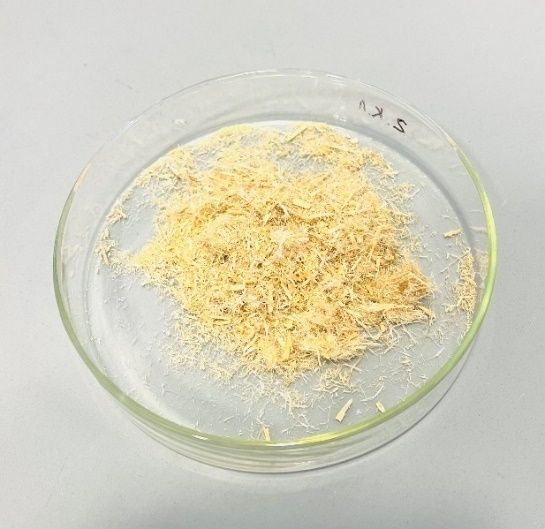
\includegraphics[width=0.3\textwidth]{assets/80}
	\caption*{Рис. 5 - Обесцвеченная целлюлоза}
\end{figure}

\begin{multicols}{2}
Анализируя результаты опыта, приведенные в таблице, можно заметить, что
выход целлюлозы увеличивается с увеличением концентрации щелочи и
времени варки. Поэтому степень делигнификации также выше.

По данным опыта максимальный выход целлюлозы составил 38,9\%. Эта
величина была определена при экстракции стеблей хлопчатника 20\%
раствором гидроксида натрия под высоким давлением (1,5 бар) и в течение
длительного времени (4 часа) при температуре 120°С. А минимальный выход
целлюлозы составляет 31,8\%, что достигается при следующих условиях
кипения: концентрация активной щелочи 10\%, температура 120°С, время 2
часа.

\emph{3. Процесс обесцвечивания целлюлозы}

Полученную сырую целлюлозу после экспериментов смешивали с 3\% раствором
H\textsubscript{2}O\textsubscript{2} в соотношении 2:1 и проводили
процесс обесцвечивания на водяной бане при температуре 80°С в течение 3
часов.

После дальнейшего обесцвечивания сырой мякоти стеблей хлопчатника
раствором перекиси водорода пробу тщательно фильтруют через
фильтровальную бумагу и промывают водой до нейтральной реакции. После
тщательной промывки образца его сушат в конвекционной печи при
температуре 105°С до постоянной массы и хранят в эксикаторе для
дальнейших исследований.

\emph{4. Исследование целлюлозы методом ИК-Фурье спектроскопии}

Методом ИК-Фурье спектроскопии определяли структуру и чистоту
делигнифицированной целлюлозы, полученной из стеблей хлопчатника методом
щелочной варки. Образец смешивали с ультрачистым бромидом калия в
соотношении 10:1 таблеточным методом и регистрировали ИК-спектры с
помощью ИК-Фурье-спектрометра IR Spirit (Shimadzu, Япония). Полученную
спектрограмму (рисунок 6) анализировали путем сравнения ее с полосами
(пиками) спектрограммы исходного образца (рисунок 3) с использованием
специальных атласов и различных литератур.
\end{multicols}

\begin{figure}[H]
	\centering
	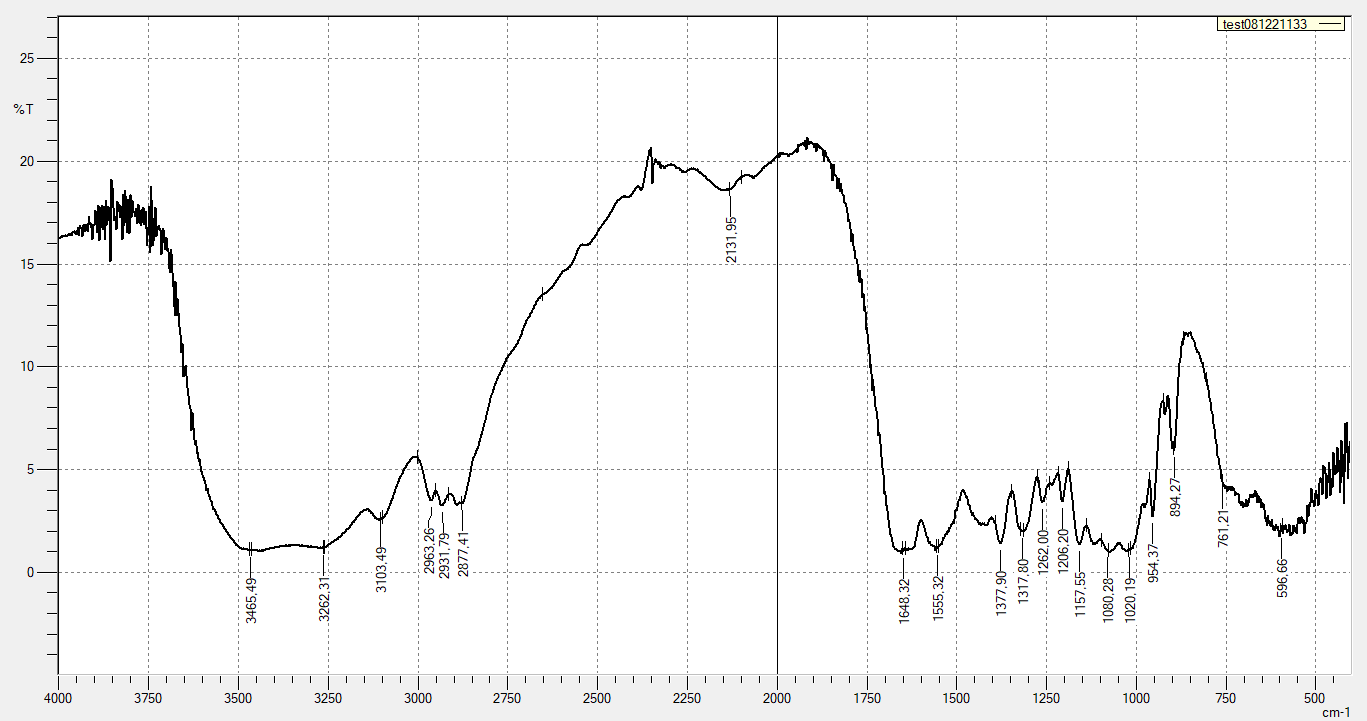
\includegraphics[width=0.8\textwidth]{assets/81}
	\caption*{Рис. 6 - Спектрограмма целлюлозы, полученной путем щелочной варки}
\end{figure}

\begin{multicols}{2}
До щелочной варки в ИК-спектрах стеблей хлопчатника наблюдаются
характерные пики, соответствующие функциональным группам, присутствующим
в целлюлозе, гемицеллюлозе, лигнине и других компонентах стебля. На
спектрограмме интенсивные полосы в области 3200-3600
см\textsuperscript{-1} соответствуют длинным колебаниям О-Н -
гидроксильных групп целлюлозы. А полосы между 2900-3000
см\textsuperscript{-1} зафиксированы как обусловленные длинными
колебаниями C-H. Полосы 1640-1660 см\textsuperscript{-1} демонстрируют
длинные колебания С=О, характерные для целлюлозы. Соответствующие
валентные колебания, указывающие на эфирную связь С-О-С, с интенсивными
полосами в районе около 1050-1150 см\textsuperscript{-1}. На наличие
гемицеллюлозы указывают полосы 1730-1740 см\textsuperscript{-1},
соответствующие ацетильным и эфирным группам, и полосы 1200-1300
см\textsuperscript{-1}, относящиеся к валентным колебаниям С-О в
гемицеллюлозе. Пики в диапазоне 1500-1700 см\textsuperscript{-1}
представляют собой ароматические скелетные колебания, характерные для
лигнина, а интенсивная полоса около 1510 см\textsuperscript{-1}
соответствует валентным колебаниям С=С. Пики в диапазоне 2800-2900
см\textsuperscript{-1} признаны связанными с липидами и восками.

В свою очередь, после щелочной варки ИК-спектры претерпевают изменения
за счет удаления гемицеллюлозы, лигнина и других компонентов. Пики
растяжения O-H остаются, но могут расширяться в области 3200-3600
см\textsuperscript{-1} из-за увеличения доступности гидроксильных групп
после удаления гемицеллюлозы и лигнина. Как уже говорилось выше, чистая
молекула целлюлозы обладает способностью поглощать воду. Длинные пики
C-H также остаются относительно неизменными. Полоса валентных колебаний
С=О в области полос 1560-1648 см\textsuperscript{-1} более выражена за
счет подавления других интерферирующих полос. Полосы, относящиеся к
гемицеллюлозе, в частности пики около 1730-1740 см\textsuperscript{-1},
уменьшаются или полностью исчезают, как и валентные колебания С=O,
связанные с гемицеллюлозой. Пики в области 1500-1700
см\textsuperscript{-1}, связанные с лигнином, особенно колебания
ароматического скелета, уменьшаются или исчезают, что указывает на
очистку от лигнина. Пик при 1510 см\textsuperscript{-1} менее заметен
или вообще исчезает. Поскольку образец предварительно не очищался
специальным образом от масел и восков, на нем могут наблюдаться следы их
характерных разводов.

В целом ИК-спектры стеблей хлопчатника до и после щелочной варки
демонстрируют существенные различия с уменьшением пиков, связанных с
нецеллюлозными компонентами в постэкстракционном спектре, что указывает
на содержание чистой целлюлозы.

\emph{5. Определение степени делигнификации целлюлозы. Определение числа
Каппа}

Число Каппа является показателем степени делигнификации целлюлозы или
обесцвечиваемости целлюлозы. Определение числа Каппа целлюлозы проводили
методом титрования по международному стандарту ISO 302:2015 «Целлюлоза.
Определение числа Каппа». Настоящий международный стандарт
распространяется на все виды химической и полухимической целлюлозы с
числом Каппа в диапазоне от 1 до 100.
\end{multicols}

\begin{table}[H]
\caption*{Таблица 2 - Число Каппа и остаточное содержание лигнина в целлюлозе}
\begin{tabular}{|l|l|l|l|l|l|l|}
\hline
№ &
  Метод получения целлюлозы &
  \begin{tabular}[c]{@{}l@{}}Концентрация \\ щелочи, \%\end{tabular} &
  \begin{tabular}[c]{@{}l@{}}Время \\ варки, ч.\end{tabular} &
  \begin{tabular}[c]{@{}l@{}}Выход \\ целлюлозы, \%\end{tabular} &
  \begin{tabular}[c]{@{}l@{}}Число \\ Каппа\end{tabular} &
  \begin{tabular}[c]{@{}l@{}}Лигнин,\\  \%\end{tabular} \\ \hline
1  & \begin{tabular}[c]{@{}l@{}}Получение целлюлозы \\ интегрированным методом \\ экстракции и делигнификации\end{tabular} & 20 & 2                  & 46,8 & 25,4 & 3,38 \\ \hline
2  & \multirow{9}{*}{\begin{tabular}[c]{@{}l@{}}Получение целлюлозы путем \\ щелочной варки\end{tabular}}                  & 10 & \multirow{3}{*}{2} & 31,8 & 42,3 & 5,58 \\ \cline{1-1} \cline{3-3} \cline{5-7} 
3  &                                                                                                                       & 15 &                    & 34,2 & 31,5 & 4,16 \\ \cline{1-1} \cline{3-3} \cline{5-7} 
4  &                                                                                                                       & 20 &                    & 35,7 & 29,8 & 3,97 \\ \cline{1-1} \cline{3-7} 
5  &                                                                                                                       & 10 & \multirow{3}{*}{3} & 32,8 & 43   & 5,73 \\ \cline{1-1} \cline{3-3} \cline{5-7} 
6  &                                                                                                                       & 15 &                    & 35,4 & 29,5 & 3,93 \\ \cline{1-1} \cline{3-3} \cline{5-7} 
7  &                                                                                                                       & 20 &                    & 37,1 & 27,2 & 3,63 \\ \cline{1-1} \cline{3-7} 
8  &                                                                                                                       & 10 & \multirow{3}{*}{4} & 33,2 & 35,6 & 4,74 \\ \cline{1-1} \cline{3-3} \cline{5-7} 
9  &                                                                                                                       & 15 &                    & 36,5 & 30,1 & 4,01 \\ \cline{1-1} \cline{3-3} \cline{5-7} 
10 &                                                                                                                       & 20 &                    & 38,9 & 28,7 & 3,83 \\ \hline
\end{tabular}
\end{table}

\begin{multicols}{2}
Таким образом, как видно из таблицы 4, хотя выход целлюлозы в опыте №5
был низким, число Каппа показало наибольшее значение - 43,0. Число Каппа
показало наименьшее значение в опыте №1 с высоким выходом целлюлозы. Это
показывает обратную зависимость между выходом и числом Каппа: более
высокий выход обычно указывает на меньшее количество лигнина в пульпе,
что способствует более эффективному выделению целлюлозы. Более высокое
значение числа Каппа, в свою очередь, указывает на повышенное содержание
лигнина в целлюлозе, что требует большего количества перекиси водорода
для эффективного отбеливания. Например, в эксперименте №1 при
максимальном выходе целлюлозы 46,8\% число Каппа составляет 25,4 при
120°C, времени кипения 2 часа и давлении 1,5 бар. Такие параметры
являются благоприятными, поскольку процесс отбеливания целлюлозы
проходит успешно.

5. \emph{Материальный баланс и пути утилизации, участвующих реагентов в технологическом процессе}

В рамках технологического процесса переработки стеблей хлопчатника в
целлюлозу особое внимание уделяется не только эффективности получаемого
продукта, но и рациональному использованию реагентов, а также их
утилизации. В таблице ниже представлены основные этапы процесса,
включающие входящие материалы, получаемые продукты и методы утилизации
реагентов, участвующих в технологическом переделе.
\end{multicols}


\begin{longtable}[c]{|p{0.12\textwidth}|p{0.12\textwidth}|l|p{0.13\textwidth}|l|p{0.3\textwidth}|}
\caption*{Таблица 3 - Материальный баланс и пути утилизации, участвующих реагентов в технологическом процессе получения 38,9 г целлюлозы} \\
\hline
Этап процесса &
  Входящие материалы &
  Масса &
  Выходящие продукты &
  Масса &
  Утилизация реагентов \\ \hline
\endfirsthead
%
\endhead
%
Экстракция масел и восков &
  Стебли хлопчатника &
  100 г &
  Стебли после экстракции &
  96,4 г &
  Хлороформ регенерируется и повторно используется путем ректификации или дистилляции. \\ \hline
 &
  Хлороформ &
  200 мл &
  Масла и воски &
  3,6 г &
  Остатки масел и восков собираются и утилизируются согласно требованиям охраны окружающей среды. \\ \hline
Кислотная обработка (HCl) &
  Стебли после экстракции &
  96,4 г &
  Очищенные стебли &
  90 г &
  Отработанная кислота нейтрализуется щелочью (NaOH), после чего образовавшиеся растворы могут быть переработаны или безопасно утилизированы в соответствии с экологическими нормами. \\ \hline
 &
  2 н HCl &
  200 г &
  Отработанная кислота &
  200 г &
   \\ \hline
Щелочная варка (NaOH) &
  Очищенные стебли &
  90 г &
  Целлюлоза &
  38,9 г &
  Отработанный раствор NaOH нейтрализуется кислотой (HCl). Образовавшиеся соли (NaCl) отделяются через фильтрацию или испарение, а вода очищается и возвращается в процесс. \\ \hline
 &
  20\% раствор NaOH (100 г NaOH + 400 г воды) &
  500 г &
  Лигнин, примеси, отходы &
  51,1 г &
   \\ \hline
Обесцвечи-вание (H₂O₂) &
  Целлюлоза &
  38,9 г &
  Обесцвеченная целлюлоза &
  38,9 г &
  Отработанный раствор H₂O₂ разлагается до воды и кислорода, минимизируя экологическое воздействие. Вода может быть повторно использована в технологическом процессе. \\ \hline
 &
  3\% H₂O₂ &
  77,8 г &
  Отработанный раствор H₂O₂ &
  77,8 г &
   \\ \hline
\end{longtable}

\begin{multicols}{2}
Утилизация и экологические меры в технологическом процессе переработки
стеблей хлопчатника в целлюлозу направлены на минимизацию воздействия на
окружающую среду и обеспечение устойчивости производства. После
экстракции масел и восков хлороформ подлежит регенерации с
использованием процесса дистилляции, что позволяет повторно применять
растворитель в последующих циклах. Остатки масел и восков утилизируются
в соответствии с экологическими стандартами. Соляная кислота (HCl),
использованная для обработки стеблей хлопчатника, нейтрализуется щелочью
(NaOH), а полученные соли, такие как NaCl, могут быть использованы
повторно или безопасно утилизированы. Растворы щелочи после варки также
нейтрализуются кислотой, а образовавшиеся отходы, включая соли и воду,
проходят очистку и, по возможности, возвращаются в производственный
цикл. Перекись водорода (H₂O₂), используемая в процессе обесцвечивания,
разлагается на воду и кислород, что делает процесс безопасным для
окружающей среды. Вода, полученная в результате разложения, может быть
использована повторно.

Эти меры направлены на минимизацию воздействия на окружающую среду и
обеспечивают устойчивость технологического процесса переработки стеблей
хлопчатника в целлюлозу.

\emph{7. Материальный баланс для получения 1 кг целлюлозы из стеблей
хлопчатника}

Материальный баланс для получения 1 кг целлюлозы из стеблей хлопчатника
предоставляет детализированное представление о расходе и выходе
материалов на каждом этапе процесса. В ходе расчета были рассмотрены все
основные входящие и выходящие материалы, включая стебли хлопчатника,
гидроксид натрия, соляную кислоту, хлороформ и перекись водорода.

Расчет для получения 1 кг целлюлозы:

1. \emph{Стебли хлопчатника:}

Выход целлюлозы составляет 38,9\% от массы исходного сырья.

Чтобы получить 1 кг целлюлозы, необходимо:

\[\frac{1\ кг}{0,389} \approx 2,57\ кг\ стеблей\]

2. \emph{Гидроксид натрия (NaOH):}

Для обработки 2,57 кг стеблей в 20\% растворе NaOH потребуется:

Масса раствора NaOH:

\[2,57\ кг\  \times 5 = 12,85\ кг\]

В растворе NaOH содержится 20\% NaOH, следовательно:

\[Масса\ чистого\ \ NaOH\  = 12,85\ кг\  \times 0,2\  = 2,57\ кг\]

Оставшаяся масса - это вода:

\[Масса\ воды\  = 12,85\ кг\  - 2,57\ кг\  = 10,28\ кг\]

3. \emph{Соляная кислота (HCl):}

Для обработки 2,57 кг стеблей требуется 2 н HCl:

≈ 5,14~кг~кислоты

4. \emph{Хлороформ:}

Для экстракции масел и восков из 2,57 кг стеблей потребуется:

≈ 5,14~л~хлороформа

5. \emph{Перекись водорода (H₂O₂):}

Для обесцвечивания 1 кг целлюлозы необходимо:

2 кг (3\% раствора H₂O₂).
\end{multicols}

\begin{table}[H]
\caption*{Таблица 4 - Сводная таблица материального баланса}
\centering
\begin{tabular}{|p{0.12\textwidth}|p{0.12\textwidth}|l|p{0.2\textwidth}|l|}
\hline
Этап процесса & Входящие материалы & Масса & Выходящие продукты & Масса \\ \hline
Экстракция масел и восков & Стебли хлопчатника & 2,57 кг & Стебли после экстракции & 2,48 кг \\ \hline
 & Хлороформ & 5,14 л & Масла и воски & 0,09 кг \\ \hline
Кислотная обработка (HCl) & Стебли после экстракции & 2,48 кг & Очищенные стебли & 2,31 кг \\ \hline
 & 2 н HCl & 5,14 кг & Отработанная кислота & 5,14 кг \\ \hline
Щелочная варка (NaOH) & Очищенные стебли & 2,31 кг & Целлюлоза & 1 кг \\ \hline
 & 20\% раствор NaOH (в составе 12,85 кг раствора) & 12,85 кг & Лигнин, примеси, отходы & 1,31 кг \\ \hline
Обесцвечи-вание (H₂O₂) & Целлюлоза & 1 кг & Обесцвеченная целлюлоза & 1 кг \\ \hline
 & 3\% H₂O₂ & 2 кг & Отработанный раствор H₂O₂ & 2 кг \\ \hline
\end{tabular}
\end{table}

\begin{table}[H]
\caption*{Таблица 5 - Итоговый материальный баланс}
\centering
\begin{tabular}{|l|l|}
\hline
Входящие материалы      & Масса (кг) \\ \hline
Стебли хлопчатника      & 2,57       \\ \hline
NaOH (чистый)           & 2,57       \\ \hline
HCl (2 н)               & 5,14       \\ \hline
Хлороформ               & 5,14       \\ \hline
Перекись водорода (3\%) & 2          \\ \hline
\end{tabular}
\end{table}

\begin{multicols}{2}
Материальный баланс для получения 1 кг целлюлозы из стеблей хлопчатника
показывает, что для производства 1 кг целлюлозы необходимо 2,57 кг
стеблей хлопчатника. Процесс включает использование 12,85 кг 20\%
раствора NaOH, 5,14 кг соляной кислоты, 5,14 л хлороформа и 2 кг 3\%
раствора перекиси водорода. В результате обработки стеблей после
экстракции образуются 0,09 кг масел и восков, а также 1 кг целлюлозы.
Отходы, включая лигнин и примеси, составляют 1,31 кг. Важным аспектом
является правильное управление отходами и отработанными растворами для
минимизации их воздействия на окружающую среду.

Таким образом, материальный баланс показывает, что процесс получения
целлюлозы из стеблей хлопчатника эффективен с точки зрения конверсии
исходного сырья в конечный продукт. Важно обеспечить правильное
управление отходами и отработанными растворами для минимизации
негативного воздействия на окружающую среду и соблюдения экологических
стандартов.
\end{multicols}

\begin{table}[H]
\caption*{Таблица 6 - Выходящие продукты и отходы}
\centering
\begin{tabular}{|l|l|l|}
\hline
Выходящие продукты и отходы & Масса (кг) & Примечания                           \\ \hline
Целлюлоза                   & 1          & Финальный продукт                    \\ \hline
Лигнин и примеси            & 1,31       & Образуется после варки               \\ \hline
Масла и воски               & 0,09       & Образуется после экстракции          \\ \hline
Отработанная кислота (HCl)  & 5,14       & Образуется после кислотной обработки \\ \hline
Отработанный раствор H₂O₂   & 2          & Образуется после обесцвечивания      \\ \hline
\end{tabular}
\end{table}

\begin{table}[H]
\caption*{Таблица 7 - Суммарная масса отходов}
\centering
\begin{tabular}{|l|l|}
\hline
Отходы                     & Масса (кг)    \\ \hline
Лигнин и примеси           & 1,31          \\ \hline
Масла и воски              & 0,09          \\ \hline
Отработанная кислота (HCl) & 5,14          \\ \hline
Отработанный раствор H₂O₂  & 2             \\ \hline
\textbf{Итого}             & \textbf{8,54} \\ \hline
\end{tabular}
\end{table}

\begin{multicols}{2}
{\bfseries Выводы.} Казахстан является одним из крупнейших производителей
хлопчатника в мире, и большая часть его производства сосредоточена в
южных регионах страны. В частности, в Туркестанской области. Это создает
значительный потенциал использования стеблей хлопчатника для переработки
и производства таких ценных продуктов, как лигноцеллюлоза и целлюлоза.
Являясь наиболее распространенным и возобновляемым источником,
лигноцеллюлоза является потенциальным сырьем для производства
дорогостоящего топлива и химикатов. Проведен ряд исследований и
определен производственный потенциал с целью переработки хлопковых
отходов, имеющих высокое содержание целлюлозы, и получения из них
ценного продукта. Кроме того, при производстве чистой целлюлозы из
стеблей хлопчатника в ходе эксперимента был апробирован ряд методов и
инновационных идей, позволяющих добиться ее высокого выхода.

Интегрирование метода предварительного обезжиривания органическим
растворителем к методу щелочной варки, который является классическим
методом извлечения целлюлозы из стеблей хлопчатника, было признано
инновационным шагом в увеличении его выхода. Ведь в ходе экспериментов
его валовой выход составил 46,8\%. Это значительно более высокий выход,
чем при классическом методе.

При обычной щелочной варке максимальный выход целлюлозы составил 38,9\%.
Это значение было известно при варке стеблей хлопчатника 20\%
гидроксидом натрия при высоком давлении (1,5 бар) и длительном времени
(4 часа) при температуре 120°С. А минимальный выход целлюлозы составляет
31,8\%, что достигается при следующих условиях заваривания: концентрация
активной щелочи составляет 10\%, температура - 120°C, а время - 2
часа. Кроме того, анализируя результаты эксперимента, можно заметить,
что по мере увеличения концентрации щелочи и времени варки увеличивается
выход целлюлозы. Следовательно, степень делигнификации также показывает
гораздо более высокий показатель.

Чистота целлюлозы, полученная в ходе экспериментов, оценивалась по двум
параметрам: ИК-Фурье спектроскопия и оценка степени делигнификации по
определению числа Каппа. В ИК-спектроскопическом методе полученная в
ходе эксперимента целлюлоза оценивалась по полосам, видимым в ИК-зоне
исходного образца, и характеризовалась уменьшением интенсивности полос,
указывающих на неспецифические функциональные группы целлюлозы,
наблюдаемые в исходном образце, или их полным исчезновением. А в
представлении результатов, полученных методом определения степени
делигнификации по числу Каппа, можно сформировать следующую гипотезу:
«Существует обратная пропорциональная зависимость между выходом
целлюлозы и числом Каппа. Он отмечает, что высокий выход обычно
указывает на небольшое количество лигнина в целлюлозе, что способствует
эффективному выделению целлюлозы. Увеличение значения числа Каппа, в
свою очередь, указывает на большее количество лигнина в целлюлозе, что
требует большего количества перекиси водорода для эффективного процесса
отбеливания». Таким образом, чем меньше значение числа Каппа, тем больше
выход целлюлозы.

По результатам материального баланса, для получения 1 кг целлюлозы
требуется 2,57 кг стеблей хлопчатника. В процессе производства
используются 12,85 кг 20\% раствора NaOH, 5,14 кг соляной кислоты, 5,14
л хлороформа и 2 кг 3\% перекиси водорода. Из стеблей после экстракции
выделяется 0,09 кг масел и восков, а конечный выход - 1 кг целлюлозы.
Отходы, такие как лигнин и примеси, составляют 1,31 кг. Важно эффективно
управлять отходами и отработанными растворами, чтобы снизить их
экологическое воздействие.

Таким образом, переработка стеблей хлопчатника и других отходов в
лигноцеллюлозу и целлюлозу может стать источником новых экономических
возможностей как для мира, так и для региона, где хлопчатник интенсивно
культивируется. Создание заводов по производству этих продуктов
неизбежно способствует созданию рабочих мест и привлечению инвестиций.
Развитие переработки стеблей хлопчатника дает значительные усилия по
диверсификации экономики региона. Вместо того, чтобы полагаться только
на экспорт сырья, Казахстан должен начать увеличивать стоимость своей
продукции, что, как известно, сделает ее экономику более устойчивой.

Переработка стеблей хлопчатника и других его отходов может помочь
сократить количество отходов, которые обычно выбрасываются в виде мусора
или сжигаются массово после сбора хлопчатника. Решением этих проблем
может быть переработка этих отходов и извлечение из них ценных
продуктов, чтобы избежать глобального потепления и других негативных
последствий для окружающей среды.

Данная научная работа является исследовательской и посвящена изучению и
сравниванию различных эффективных способов получения целлюлозы из
стеблей хлопчатника, который выращивается в Туркестанской области.
\end{multicols}

\begin{center}
{\bfseries References}
\end{center}

\begin{noparindent}
1.
  Shatalov A.A., Pereira H. Xylose production from giant reed (Arundo
  donax L.): Modeling and \\optimization of dilute acid hydrolysis
  //Carbohydrate Polymers. -2012. - Vol. 87(1). -P. 210-217. DOI:

  10.1016/j.carbpol.2011.07.041

2.
  Mohanty A. K., Misra M., Drzal L. T. (ed.). Natural fibers,
  biopolymers, and biocomposites. - CRC press, 2005.
  DOI:10.1201/9780203508206

3.
  Narayan R. Biodegradable/compostable plastics. - 2005. -P. 28-35.

4.
  Akdeniz R. C., Acaroglu M., Hepbasli A. Cotton stalk as a potential
  energy source //Energy sources. - 2004. - Vol. 261. - P. 65-75.

5.
  Gomes R. S. et al. Cotton (Gossypium) plant residue for industrial
  fuel.: An economic assessment //Industrial crops and products. -
  1997. - Vol. 7(1). - P. 1-8.

6.
  Li G. et al. Properties study of cotton stalk fiber/gypsum composite
  //Cement and Concrete Research. - 2003. - V. 33(1). - P. 43-46.
  DOI:10.1016/S0008-8846(02)00915-8

7.
  Du S. et al. High-pressure assist-alkali pretreatment of cotton stalk
  and physiochemical characterization of biomass //Bioresource
  technology. - 2013. - Vol. 148. - P. 494-500.
  DOI:~10.1016/j.biortech.2013.09.020

8.
  Silverstein R. A. et al. A comparison of chemical pretreatment methods
  for improving saccharification of cotton stalks //Bioresource
  technology. - 2007. - Vol. 98(16). - P. 3000-3011.

  DOI:10.1016/j.biortech.2006.10.022

9.
  Rehman M. S. U. et al. Optimization of sono-assisted dilute sulfuric
  acid process for simultaneous pretreatment and saccharification of
  rice straw //International Journal of Environmental Science and
  \\Technology. - 2014. - Vol. 11. - P. 543-550.
  DOI:10.1007/s13762-013-0294-0

10.
  Kapoor M. et al. Structural features of dilute acid, steam exploded,
  and alkali pretreated mustard stalk and their impact on enzymatic
  hydrolysis //Carbohydrate polymers. - 2015. - Vol. 124. - P.
  265-273. DOI:10.1016/j.carbpol.2015.02.044

11.
  Cao X. et al. Comparative study of the pyrolysis of lignocellulose and
  its major components: \\Characterization and overall distribution of
  their biochars and volatiles //Bioresource technology. - 2014. -
  Vol. 155. - P. 21-27. DOI: 10.1016/j.biortech.2013.12.006

12.
  Al Shra'ah A., Helleur R. Microwave pyrolysis of cellulose at low
  temperature //Journal of Analytical and Applied Pyrolysis. - 2014. -
  Vol. 105. - P. 91-99. DOI: 10.1016/j.jaap.2013.10.007

13.
  Lin T., Goos E., Riedel U. A sectional approach for biomass: Modelling
  the pyrolysis of cellulose //Fuel processing technology. - 2013. -
  V. 115. - P. 246-253. https://doi.org/10.1016/j.fuproc.2013.03.048

1.
  Li J. et al. Characteristics and deoxy-liquefaction of cellulose
  extracted from cotton stalk //Fuel. - 2016. - V. 166. - P. 196-202.
  DOI:10.1016/j.fuel.2015.10.115
\end{noparindent}

\emph{{\bfseries Сведения об авторах}}

\begin{noparindent}
Куртибай Қ.А. - магистрант, научный сотрудник ТОО
«Научно-производственный центр экологической и промышленной
биотехнологии», Астана, Казахстан, e-mail: kurtibayqb@gmail.com;

Қаппасұлы Ә. - магистр техники и технологии, научный сотрудник ТОО
«Научно-производственный центр экологической и промышленной
биотехнологии», Астана, Казахстан, e-mail: kappasuly@mail.ru;

ҮсеноваА.Ә.- магистр естествознания, генеральный директор ТОО
«Научно-производственный центр экологической и промышленной
биотехнологии», Астана, Казахстан, e-mail: ussenovaaall@gmail.com;

Жатканбаев Е.Е. - д.т.н., ассоциированный профессор, Казахский
университет технологии и бизнеса имени К. Кулажанова, Астана, Казахстан,
e-mail: erlan.ntp@mail.ru;

Жатканбаева Ж.К. - к.х.н., доцент, Евразийский Национальный Университет
имени Л.Н. Гумилева, Астана, Казахстан, e-mail: zhanna01011973@mail.ru;

Молдагулова Н.Б. - к.в.н, ведущий научный сотрудник ТОО
«Научно-производственный центр экологической и промышленной
биотехнологии», Астана, Казахстан, e-mail: m\_nazira1967@mail.ru;

Молдагулова Э.Б. - младший научный сотрудник ТОО
«Научно-производственный центр экологической и промышленной
биотехнологии», Астана, Казахстан, e-mail:
molgagulova\_elmira1968@mail.ru.
\end{noparindent}

\emph{{\bfseries Information about the authors}}

\begin{noparindent}
Kurtibay K.A. - Master\textquotesingle s student, Research Associate of
«Scientific and Production Center of Ecological and Industrial
Biotechnology» LLP, Astana, Kazakhstan, e-mail: kurtibayqb@gmail.com;

Kappassuly A. - Master of Engineering and Technology, Research
Associate, «Scientific and Production Center of Ecological and
Industrial Biotechnology» LLP, Astana, Kazakhstan, e-mail:
kappasuly@mail.ru;

Ussenova A.A. - Master of Natural Sciences, General Director,
«Scientific and Production Center of Ecological and Industrial
Biotechnology» LLP, Astana, Kazakhstan, e-mail: ussenovaaall@gmail.com;

Zhatkanbayev Ye.Ye. - Doctor of Technical Sciences, Associate Professor,
Kazakh University of Technology and Business named after K. Kulazhanov,
Astana, Kazakhstan, e-mail: erlan.ntp@mail.ru;

Zhatkanbayeva Zh.K. - Candidate of Chemical Sciences, Associate
Professor, L.N. Gumilev Eurasian National University, Astana,
Kazakhstan, e-mail: zhanna01011973@mail.ru;

Moldagulova N.B. - Candidate of Veterinary Sciences, Leading Researcher,
«Scientific and Production Center of Ecological and Industrial
Biotechnology» LLP, Astana, Kazakhstan, e-mail:

m\_nazira1967@mail.ru.

E.B. Moldagulova - junior researcher, «Scientific and Production Center
of Ecological and Industrial Biotechnology» LLP, Astana, Kazakhstan,
e-mail: molgagulova\_elmira1968@mail.ru.
\end{noparindent}
